% Preamble {{{
\documentclass[11pt,a4paper,titlepage,dvipsnames,cmyk]{scrartcl}
\usepackage[english]{babel}
\typearea{12}
% }}}

% Set indentation and line skip for paragraph {{{
\setlength{\parindent}{0em}
\setlength{\parskip}{1em}
\usepackage[margin=2cm]{geometry}
\addtolength{\textheight}{-1in}
\setlength{\headsep}{.5in}
% }}}

\usepackage{hhline}
\usepackage[table]{xcolor}
\usepackage{mathtools}
\usepackage[T1]{fontenc}

% Headers setup {{{
\usepackage{fancyhdr}
\pagestyle{fancy}
\lhead{Information Processing and the Brain}
\rhead{Josh Felmeden}
\usepackage{hyperref}
% }}}

% Listings {{{
\usepackage[]{listings}
\lstset
{
    breaklines=true,
    tabsize=3,
    showstringspaces=false
}

\definecolor{lstgrey}{rgb}{0.05,0.05,0.05}
\usepackage{listings}
\makeatletter
\lstset{language=[Visual]Basic,
backgroundcolor=\color{lstgrey},
frame=single,
xleftmargin=0.7cm,
frame=tlbr, framesep=0.2cm, framerule=0pt,
basicstyle=\lst@ifdisplaystyle\color{white}\footnotesize\ttfamily\else\color{black}\footnotesize\ttfamily\fi,
captionpos=b,
tabsize=2,
keywordstyle=\color{Magenta}\bfseries,
identifierstyle=\color{Cyan},
stringstyle=\color{Yellow},
commentstyle=\color{Gray}\itshape
}
\makeatother
\renewcommand{\familydefault}{\sfdefault}
\newcommand{\specialcell}[2][c]{%
\begin{tabular}[#1]{@{}c@{}}#2\end{tabular}}
% }}}

% Other packages {{{
\usepackage{graphicx}
\graphicspath{ {./pics/} }
\usepackage{needspace}
\usepackage{tcolorbox}
\usepackage{soul}
\usepackage{babel,dejavu,helvet}
\usepackage{amsmath}
\usepackage{amssymb}

\usepackage{booktabs}
\usepackage{tcolorbox}
\usepackage[symbol]{footmisc}
\renewcommand{\thefootnote}{\fnsymbol{footnote}}
\renewcommand{\familydefault}{\sfdefault}
\usepackage{enumitem}
\setlist{nolistsep}
% }}}

% tcolorbox {{{
\newtcolorbox{blue}[3][] {
colframe = #2!25,
colback = #2!10,
#1,
}

\newtcolorbox{titlebox}[3][] {
colframe = #2!25,
colback = #2!10,
coltitle = #2!20!black,
title = {#3},
fonttitle=\bfseries
#1,
}
% }}}

% Title {{{
\title{Information Processing and the Brain}
\author{Josh Felmeden}
% }}}

\begin{document}
\maketitle
\tableofcontents
\newpage
\section{Information Theory}
Information theory quantifies the amount of information that is potentially available from the communication channel using. So, we look to answer the question: can the receiver decide how informative the channel is likely to be; how much information is in the channel.

\subsection{Randomness}
The key is that if the information in the channel is predictable, the receiver is not going to learn much from this. Therefore, we will look at randomness (coin flipping, geiger counters, etc).

We will also look and unexpectedness, and consider the relationship between randomness, unexpectedness, and information theory.

Netflix is a good example of this. Their star rating of films helps them to recommend films to you, and use your experiences to recommend films to others. The recommended tab is the \textit{channel} in the information theory. The films are the medium, and Netflix is communicating to the user information about the film. If Netflix recommends a really popular film, the information is predictable, and the user is not learning much. Therefore, we are not gaining much information about the quality of the films.

Another example is the star rating of movies. The star rating is not `random' enough for the consumer, in that there is not enough information that we as the user can learn from this. A good film with a lot of hype will likely have a good star rating, and therefore we would already know this.

Therefore, we can say that a statement, despite being correct, can be useless if we can predict it.

\begin{tcolorbox}
\textit{The theory of information starts with an attempt to allow us to quantify the informativeness of information, but not its salience or validity.}
\end{tcolorbox}

\section{Shannon's entropy}
For a finite discrete distribution with a random variable $X$, possible outcomes $\{x_1,, x_2, \dots, x_n\} \exists \mathcal{X}$ and a probability mass function $p_x$ giving probabilities $p_X(x_i)$, the entropy is:
\begin{align*}
H(X) = - \sum_{x_i \exists \mathcal{X}}p_X(x_i) \log_2 p_X(x_i)
\end{align*}

This formula \textit{quantifies} some information received. In the example of star ratings on netflix:

\begin{center}
\begin{tabular}{ll}
    \toprule
    1 star & 0.016 \\
    2 star & 0.310 \\
    3 star & 0.627 \\
    4 star & 0.057 \\ \bottomrule
\end{tabular}
\end{center}

We obtain the following formula:
\begin{align*}
H(X) = -0.016 \log_2 0.016 - 0.31 \log_2 0.31 - 0.627 \log_2 0.627 - 0.057 \log_2 0.057 \approx 1.28
\end{align*}

Choosing base two is arbitrary, but because we are dealing with information, it is useful to deal in bits. In other circumstances, it is possible to choose a different base. The result, $1.28$ is the entropy for the channel of Netflix film star ratings.

If the star ratings were all equally likely, we would get an entropy of:
\begin{align*}
H(X) = -4 \times 0.25 \log_2 0.25 = 2
\end{align*}

This is higher value entropy meaning the information is more useful.

In contrast, if all films are rated one star, we end up with entropy 0, meaning that it is useless. We assume $\log 0$ is 0 for shannon's entropy despite this not being the case in reality.

\subsection{Nice properties}
Shannon's entropy works on any sample space. It's good because you can calculate this on things that would otherwise be impossible, such as items bought from a grocers. This is because it is defined on probability space, while other calculations are calculated in vector space (such as mean, etc).

It's \textbf{always positive}, unless it is zero, which is when the distribution \textit{isn't random} (aka \textit{determined}).

If the distribution is \textit{uniform}:
\begin{align*}
p_X(x_i) = \frac{1}{n}
\end{align*}

for all $x_i$ where ($\#$ is equivalent to \texttt{len})
\begin{align*}
n = \#\mathcal{X}
\end{align*}

then, since $-\log_2(1/n) = \log_2n$
\begin{align*}
H(X) = \log_2n
\end{align*}

We won't prove it here, but is not difficult to prove that:
\begin{align*}
0 \le H(X) \le \log_2n
\end{align*}

with $H(X) = 0$ \textit{only} if one probability is one and the rest zero, and $H(X) = \log_2 n$.

\subsubsection{Case of n = 2}
With two outcomes, $a$ and $b$ with $p(a) = p$ and $p(b) = 1-p$ then
\begin{align*}
H = -p\log_2 p-(1-p)\log_2(1-p)
\end{align*}

The resulting graph of entropy will be symmetric; rising towards 1.

\subsubsection{Source coding}
the main reason to believe that Shannon's entropy is a good quantity for calculating entropy is its relationship to so called source coding.

Consider storing a long sequence of letters \texttt{A, B, C, D} as binary (\texttt{AABACBDA} for example). If we wanted to digitise this, we might use a very simple binary representation of these characters (\texttt{A = 00, B = 01, ...}). Using this representation means the average bits per letter is 2. Now, if we had different distribution of letters, then we could possibly come up with a smaller, more compact version of the code. For example, if we had the following distribution:
\begin{center}
    \begin{tabular}{cccc}
        A & B & C & D \\ \midrule
        0.5 & 0.25 & 0.125 & 0.125
    \end{tabular}
\end{center}
We could use the following encoding:
\begin{center}
    \begin{tabular}{cccc}
        A & B & C & D \\ \midrule
        0 & 10 & 110 & 111
    \end{tabular}
\end{center}

Don't forget that this resulting code should be \textit{prefix free}.

Now, we can prove that this code is shorter on average:
\begin{align*}
L = 0.5 \times 1 + 0.25 \times 2 + 0.125 \times 3 + 0.125 \times 3 = 1.75 < 2
\end{align*}

This is also the same as the Shannon's entropy of the code. Each of the logs are giving us the length of the corresponding code word.

The source coding theorem states that, for the most efficient code, we get:
\begin{align*}
H(X) \le L < H(X) + 1
\end{align*}

This means that if you have a sequence of objects that have some regularity and you want to code them into binary, the channel's entropy is a lower bound on the average length of a message and you can get a \textit{prefix free} code within one of Shannon's entropy.

\subsection{Joint and Conditional Entropy}
Typically, we want to use information theory to study the relationship between two random variables. So far, we have only looked at single variables.

\begin{tcolorbox} [space to upper,
collower=white,
title={Joint Entropy},
nobeforeafter,
halign lower=flush right, ]
Given two random variables $X$ and $Y$, the probability of getting the pair $(x_i, y_j)$ is given by the \textbf{joint probability} $p(X,Y) (x_i,y_j)$. THe joint entropy is just the entropy of the join distribution:
\begin{align*}
H(X,Y) = - \sum_{i,j}p_{X, Y}(x_i, y_j)\log_2p_{X,Y}(x_i,y_j)
\end{align*}

This is essentially the probability that $x$ will produce $x_i$ and that $y$ will produce $y_j$
\end{tcolorbox}

Here's an example:
\begin{center}
    \begin{tabular}{c|cc}
        & $x_0$ & $x_1$ \\ \midrule
        $y_0$ & $1/4$ & $1/4$ \\
        $y_1$ & $1/2$ & $0$
    \end{tabular}
\end{center}

\begin{align*}
H(X,Y) = -\frac{1}{2}\log_2 \frac{1}{4} - \frac{1}{2}\log_2 \frac{1}{2} = \frac{3}{2}
\end{align*}

\subsubsection{Conditional Entropy}
$p_{X|Y}(x_i|x_j)$ is the \textbf{conditional probability} of $x_i$ given $y_j$. If we know that $Y = y_j$, it gives us the probability that the pair is $(x_i, y_j)$.

\begin{align*}
p_{X|Y}(x_i|y_j) = \frac{p_{(X,Y)}(x_i, y_j)}{p_Y(y_j)}
\end{align*}

The \textbf{marginal probability} for $x$ is: $p_X(x_i) = \sum_{j}p_{(X,Y)}(x_i,y_j)$. This is the way of getting the probabilities for one of the two random variables from the joint distribution.

Let's now substitute the conditional probability into the formula for entropy:

\begin{align*}
H(X|Y = y_j) = -\sum_ip_{(X|Y)}(x_i|y_j)\log_2 p_{X|Y}(x_i,y_j)
\end{align*}

This is the entropy of $X$ as we know $Y = y_j$. We call this the \textbf{conditioned entropy}.

The conditional entropy is the average amount of information still in $X$ when we know $Y$. It also has some pretty nice properties:

If $X,Y$ are \textit{independent}, then:
\begin{align*}
    p_{X,Y} (x_i, y_j) = p_X(x_i) p_Y(y_j)
\end{align*} 

For all $i,j$ and
\begin{align*}
p_{X|Y}(x_i|y_j) = p_X(x_i)
\end{align*}

so
\begin{align*}
H(X|Y) = -\sum_{i,j} p_{X,Y}(x_i,y_j) \log_2 p_{X|Y}(x_i|y_j) = H(X)
\end{align*}

Which is what we want, since if $Y$ tells us nothing about $X$, then the conditional entropy should just be the same as the entropy of $X$.

Conversely, if $X$ is \textit{determined} by $Y$, then $H(X|Y) = 0$. This could happen if the only $x_j,y_i$ pairs that actually occur are $(x_i,y_i)$.


\subsection{Mutual Information}
Given two (overlapping) variables, there will be some information that is shared by these two entropies, and this is called \textbf{mutual information}, and is defined as:
\begin{align*}
I(X,Y) = H(X) + H(Y) - H(X,Y)
\end{align*}

Or:
\begin{align*}
I(X,Y) = H(X) - H(X|Y) = H(Y) - H(Y|X)
\end{align*}

By substituting in the formulas, we end up with:
\begin{align*}
I(X,Y) = \sum_{i,j} p_{X,Y} (x_i, y_j) \log_2 \frac{p_{X,Y}x_i y_j}{p_X (x_j)p_Y(y_j)}
\end{align*}

Going back to the previous example:
\begin{center}
    \begin{tabular}{c|cc}
        & $x_0$ & $x_1$ \\ \midrule
        $y_0$ & $1/4$ & $1/4$ \\
        $y_1$ & $1/2$ & $0$
    \end{tabular}
\end{center}

This has $H(X,Y) = 3/2, H(X) \approx 0.81$ and $H(Y) = 1$ so $I(X,Y) \approx 0.31$

If $X$ and $Y$ are independent, we just end up with $I(X,Y) = 0$. In fact, $I(X,Y) \ge 0$

\subsection{Correlation}
The correlation is defined as:
\begin{align*}
C(X,Y) = \frac{\langle(X-\mu_X)(Y-\mu_Y)}{\sigma_X \sigma_Y}
\end{align*}

Where $\mu_X$ is the average of $X$ and $\sigma_X$ is the standard deviation.

Correlation only works if $X,Y$ take their values in vector space (meaningfully be able to multiply the two together).

Consider:
\begin{center}
    \begin{tabular}{l|lll}
        & -1 & 0 & 1 \\
        \midrule
        1 & 1/4 & 0 & 1/4 \\
        0 & 0 & 1/2 & 0
    \end{tabular}
\end{center}

Then:
\begin{align*}
C(X,Y) = 0
\end{align*}

Whereas $I(X,Y) = 1$.

\subsection{The data processing inequality}
There is something called \textbf{conditional independence}. Imagine playing a game of snakes and ladders, and $X,Y,Z$ are the resulting position after moves 1,2,3 respectively. Knowing $X$ will change the probability of $Z$, but only if we don't know $Y$, since if we know $Y$, it doesn't really matter what $X$ was. This means that $X$ and $Z$ are conditionally independent (conditioned on $Y$).

The data processing inequality states that if:
\begin{align*}
X \rightarrow Y \rightarrow Z
\end{align*}

then:
\begin{align*}
I(X,Y) \ge I(X,Z)
\end{align*}

With equality if and only if $X \rightarrow Z \rightarrow Y$

\section{Information Theory in the Brain}
\subsection{Information in the Brain}
\textit{Spike trains} are when neurons spike with some level of voltage when they are activated. This spike passes from neuron to neuron, which is how information is passed along an axon.

We can use Shannon's entropy to look at the similarities in these spikes to see the shared information.

An experiment was performed on a fly where it was shown a series of bars on a TV screen and the spike trains from the neurons at the back of the brain (the ones that observe horizontal movement) was recorded. More specifically, the timing of the spikes was recorded. This information was then \textit{discretised}, and evaluated. The information recorded are the action spikes. \textit{Discretisation} meant that the information was looked at in 3ms, and then return a 1 if there is a spike, or a 0 if not (think time bins). This binary sequence was then split up into words. Each word corresponds to the amount of time that an entire piece of information has been encoded. The calculations performed revealed that the neurons that were being looked at only remember things in 30ms, so there was a natural `word length' for splitting up the binary sequence, thus 30ms was taken.

These words can now be converted into a set of objects. The random variable that is taken as the communication channel is a chunk of spike train for 30ms, represented by one of the words. Now, we want to look at the probability of different words:
\begin{align*}
p(w_0) \approx \frac{\#(\text{occurance of } w_0)}{\# (\text{trials})}
\end{align*}

Now, two different tests were performed. The first is where the stimulus is random. The second is where a fixed five minute segment of the stimulus is shown ($H(W)$), and the responses are considered ($H(W|S)$). 

Now, we can get the mutual information about the words given:
\begin{align*}
I(W,S) = H(W) - H(W|S)
\end{align*}

Or, the information about $S$ is the total information in $W$ subtract the noise.

\subsubsection{Discretisation size}
One important question is how to decide how small to make hte discretisation time and how long to make the words. In our example, given that $\delta t = 3ms$ gives $78 \pm 5$ bits per second or $1.8 \pm 0.1$ bits per spike.

Unfortunately, if we have a 30ms word with 3ms letters, this gives us 10 letters per word giving $2^{10} = 1024$. If six seconds of data are used for the repeating stimulus, that is 100 different stimuli, then even for a three hour recording, there are 1800 trails for each stimulus. This is not a big amount for estimating 1024 probabilities.

\subsection{Differential Entropy}
\textbf{Differential Entropy} is the name given to Shannon's entropy for continuous probability distributions where the sample space is $\mathcal{X} \subseteq \mathbf{R}^d$. In the examples we will be looking at, $d = 1$. The idea is that: $h(X) = \int dxp(x) \log_2 p(x)$. This is a good guess as to what the continuous distribution would look like of Shannon's entropy.

If we consider a uniform distribution where:
\begin{align*}
p(x) = \bigg \{ \begin{matrix}
    1/a & x \in [0,a] \\
    0 & \text{otherwise}
\end{matrix}
\end{align*}

So
\begin{align*}
h(X) = \int_{-\infty}^{\infty} dx p(x) \log_2 p(x) = - \frac{1}{a}\int_{0}^{a}dx \log_2 \frac{1}{a}
\end{align*}

And so:
\begin{align*}
h(X) = \log_2 a
\end{align*}

This, unfortunately, does not guarantee that the result will be positive, which is one of the useful properties of Shannon's entropy.

\subsubsection{Gaussian distribution}
$$p(x) = \frac{1}{\sqrt{2 \pi \sigma^2}}e^{\frac{-x^2}{2\sigma^2}}$$

If we substitute and integrate by parts, we get:
$$h(x) = \frac{1}{2} \log_2 2 \pi e \sigma ^2$$

As you expand the distributions, we can prove that for fixed variance, Gaussian has the highest entropy.

Densities are not probabilities. The discrete case $p(x)$ is the probability that $X = x$. For the continuous case:
\begin{align*}
\int_{x_0}^{x_1} dx p(x)
\end{align*}

is the probability that $x_0 \le x \le x_1$. The usual sums and probabilities go to integrals and densities doesn't work because there is a $p$ in the log.

We also need to model the sensitivity of the receiver as well as the behaviour of the source.

\subsection{Relationship between Differential entropy and Shannon's entropy}
Let $\delta = x_{i+1} - x_i$. Consider the discrete random variable $X^\delta$. Now, instead of the continuous distribution we had before, we now have a discrete representation of the interval (differentiation by first principle (by faking it)). A more elegant approach to this is the \textbf{mean value theorem}. This is where you choose two heights for the histogram: the first being the lowest possible point, and the other being the highest, and then choosing the mean point of this.

\subsection{Mutual information for continuous probabilities}
The differential mutual information is:
\begin{align*}
I(X,Y) = \int p(x,y) \log_2 \frac{p(x,y)}{p(x)p(y)}
\end{align*}

And satisfies the same identities as the mutual information:
\begin{align*}
I(X,Y) = h(X) + h(Y) - h(X,Y)
\end{align*}

It has some advantages over the differential entropy; in particular, it is invariant under changes of variable in $X$ and $Y$. The differential mutual information is the same as the mutual information in the sense that, using the notation above:
\begin{align*}
I(X^{\delta x}, Y^{\delta y}) \rightarrow I(X,Y)
\end{align*}

as $\delta x$ and $\delta y$ approach zero. Furthermore,
\begin{align*}
I(X,Y)) \ge 0
\end{align*}

\subsection{Applications of differential entropy}
The sick part of entropy is its relationship to communication through the source coding theorem. At first, it might appear that there is no analogous set of ideas for differential entropy since, in a sense, the amount of information encoded in the outcome of a continuous variable must be infinite if read to infinite precision. However, of course, in real world communication, nothing is read to infinite precision and there is a theory of communication using continuous signals which includes the signal noise and imprecision of signal transmission. we won't look at this here, and instead consider the example of infomax.

\section{Infomax}
This is another information theory example we will consider. It is an approach to \textit{unmixing} data, and gives an in-principle explanation for how the brain might perform auditory source separation. In other words, it shows how source separation might be performed.

The problem is as follows: imagine you are in a crowded room (classically at a \textit{cocktail party}. Lots of people are talking, but if oyu concentrate on one voice at a time, you can separate it from the racket. The opposite effect can be observed when meditating or sitting in thoughtful silence, where we suddenly notice how loud distant noises are. These sounds are filtered without thinking. This is called auditory source separation and the question of how to do this is called the \textbf{cocktail party problem}.

The problem can be formalised. Given the sources $\mathbf{s}(t)$ where $\mathbf{s}$ is a vector over multiple sources. Now we do source separation with only two recordings, one for each ear. Here, we are just going to consider the simpler problem of source separation when there are many recordings as there are sources, we also assume the mixin is linear and instantaneous. Real mixing of auditory sources in a room will only have these properties approximately. Using this assumptions, we have:
\begin{align*}
\mathbf{r}(t) = M\mathbf{s}(t)
\end{align*}
with $M$ being a square mixing matrix. Our goal is to find the unknown source signals $\mathbf{s}(t)$ from the known recordings $\mathbf{t}$

Although it makes little difference, we will restrict ourselves to two sources, so $\mathbf{s}$ and $\mathbf{r}$ are two-dimensional vectors and $M$ is a two by two matrix.

We assume the two sources are independent $p_{s1,s2} = p_{s1}p_{s2}$; the point of source separation is to unmix independent sources. Now, we want to find the unmixing matrix $W$ so that knowing:
\begin{align*}
\mathbf{x}(t) = W\mathbf{r}(t)
\end{align*}

is as good as knowing the sources. Since we know $\mathbf{x} = WM\mathbf{s}$, we want $WM$ to be a diagonal matrix multiplied by a permutation matrix. Changing the amplitude of the source, or reordering doesn't matter. This means that
\begin{align*}
WM = \text{diag}(d_1,d_2)
\end{align*}

or
\begin{align*}
WM= \begin{pmatrix}
    0 & d_1 \\
    d_2 & 0
\end{pmatrix}
\end{align*}

where $d_1$ and $d_2$ are real numbers. Hence:
\begin{align*}
\mathbf{s} \rightarrow^\text{mixing} \mathbf{r} = M\mathbf{s} \rightarrow^\text{unmixing} \mathbf{x} = W \mathbf{r}
\end{align*}


One difficulty with looking at this problem is that it involves continuous random variables, while we have so far only looked at the discrete case. For this reason, some of the results will just be quoted. Some changes are that we get:
\begin{align*}
h(X) = -\int p(x) \log p(x) dx
\end{align*}

But it is no longer always positive.

now, the idea is to solve the problem by using the face that $S_1$ and $S_2$ are independent. We only need to find $W$ so that $X_1$ and $X_2$ are also independent. One approach could be to decorrellate the random variables:
\begin{align*}
C(X_1,X_2) = \langle (X_1 - \langle X_1\rangle)(X_2 - \langle X_2 \rangle ) \rangle _{(X_1,X_2)}
\end{align*}

where the expectation value for continuous random variable has the obvious definition:
\begin{align*}
\langle g(X) \rangle = \int p_X (x) g(x) dx
\end{align*}

It is easy to check that the correlation vanishes if $X_1$ and $X_2$ are independent, however, the flaw in this approach is that the converse is not true. It is possible to have zero correlation while still having statistical dependence.  to see this, imagine that $EX_1$ and $EX_2$ are zero and that we have chosen $W$ so that the correlation matrix is the identity:
\begin{align*}
C_ab = C(X_a, X_b) = 1
\end{align*}

It is then easy to see that rotations:
\begin{align*}
\begin{pmatrix}
    X_1' \\
    X_2'
\end{pmatrix}
= 
\begin{pmatrix}
    \cos \theta & \sin \theta \\
    =\sin \theta & \cos \theta
\end{pmatrix}
\begin{pmatrix}
    X_1 \\
    X_2
\end{pmatrix}
\end{align*}

do not change the correlation matrix. For this reason, the decorrelation prescription has a rotational ambiguity and something more is needed. That is to require that $I(X_1,X_2) = 0$ since this happens if and only if $X_1, X_2$ are independent. The problem is that $I(X_1,X_2)$ is pretty had to calculate. So, infomax basically just looks at $h(X_1,X_2)$:
\begin{align*}
I(X_1,X_2) = h(X_1) + h(X_2) - h(X_1, X_2)
\end{align*}

Maximising the joint entropy $h(X_1,X_2)$ will give a \textit{minimum} of the mutual information, meaning the variations in the individual entropies $h(X_1)$ and $h(X_2)$ can be ignored. Unfortunately, due to the possibility of trivially scaling the entropy, $X_a \rightarrow \lambda X_a$ causes the joint entropy $h(X_1, X_2) \rightarrow h(X_1,X_2) + \log |\lambda|$ so $h(X_1,X_2)$ can be made arbitrarily large by scaling, something that tells us nothing about mixing and unmixing. Inspired by the behaviour of neurons, this is solved by adding a saturation non-linearity:
\begin{align*}
y_1 = g(x_1 + w_1) \\
y_2 = g(x_2 + w_2)
\end{align*}

where
\begin{align*}
g(u) = \frac{1}{1+e^{-u}}
\end{align*}

Is a saturating non-linearity so $g : (-\infty, \infty) \rightarrow (0,1)$

This leaves us with:
\begin{align*}
\mathbf{s} \rightarrow^\text{mixing} \mathbf{r} = M\mathbf{s} \rightarrow^\text{unmixing} \mathbf{x} = W\mathbf{r} \rightarrow^\text{non-linearity} \mathbf{y} : y_a = g(x_a + w_a)
\end{align*}

From here on, we will write
\begin{align*}
y_a = g(x_a + w_a) = f(r_1,r_2:W,w_1)
\end{align*}

where $f$ is the function parameterised by $W$ and $w_a$ mapping from the recording to $y$. Before considering the source separation problem, lets look at the effect of the non-linearity on its own. We consider the one-to-one case:
\begin{align*}
r \rightarrow^\text{multiply} x = Wr \rightarrow^\text{non-linearity} y = g(x + w) = f(r;w,W)
\end{align*}

Where $W$ and $w$ are now both scalars and $r,x,y$ are outcomes for random variables $R,X,Y$. We consider maximising the entropy $h(Y)$, which maximises the information in $Y$ about $R$:
\begin{align*}
I(R;Y) = h(Y) - h(Y|R)
\end{align*}

However, $h(Y|R)$ is constant since $R$ determines $Y$. In the discrete case, we are familiar with, this would be easy to discuss since it would just be zero. In the continuous case, its not that simple. Its actually negative infinity, but the consequence is the same (it doesn't depend on $W$ and $w$). To maximise $h(Y)$ we need to calculate derivatives and these are calculable and well defined, even if the quantity being differentiated is not. In this case:
\begin{align*}
h(Y) = - \int p(y) \log p(y) dy
\end{align*}

and this is estimated by
\begin{align*}
h(y) = -\log p(y)
\end{align*}

In other words, if $n$ values of $y$ are drawn from $Y$ then
\begin{align*}
\frac{1}{n} \sum_i h(y_i) \rightarrow h(Y)
\end{align*}

as $n$ gets large.

Of course, we do not have $p_Y(y)$ and it would be difficult to estimate, but we actually don't need it to get hte derivative of $h(y)$. We have seen that already since $y = f(r;W,w)$
\begin{align*}
p_Y(y) = \frac{p_R[r = f^{-1}(y)]}{|f'(f^{-1}(y))|}
\end{align*}

so
\begin{align*}
h(y) = -\log p_R (r) + \log |f'|
\end{align*}

and $p_R(r)$ is independent of the parameters. Now, for our choice of saturating and non-linearity
\begin{align*}
g(u) &= \frac{1}{1 + \exp(-u)} \\
\frac{dg}{du} &= g(1-g)
\end{align*}

and hence
\begin{align*}
\log |f'| = \log W + \log f + \log (1-f)
\end{align*}

Now we know $f$:
\begin{align*}
f = g(Wr + w)
\end{align*}

so
\begin{align*}
\frac{df}{dW} = rf(1-f)
\end{align*}

and hence
\begin{align*}
\frac{dh(y)}{dW} = \frac{1}{W} + \frac{1}{f}rf(1-f) - \frac{1}{1-f}rf(1-f) = \frac{1}{W} + r(1-2y)
\end{align*}

Similarly
\begin{align*}
\frac{dh(y)}{dw} = 1-2y
\end{align*}

these quantities $r,y,W$ are numbers we have access to:
\begin{itemize}
    \item $W$ is a parameter,
    \item $r$ is the recorded signal
    \item we can sample $r(t)$ at a set of times to get a set of $r$s
    \item $y$ is a function of $s$.
\end{itemize}

Now, we choose a starting $W$ and $w$ and estimate the gradient and then change $W$ and $w$ a small amount, repeating until the optimum values are found. The optimum value would look like
\begin{align*}
f(r) = \int_{-\infty}^{r} p_R(u) du
\end{align*}

Now, we don't know $p_R(r)$ and we chose $f(r)$ at the start, here it is a member of a two-parameter family of functions parameterised by $W$ and $w$. Ideally, if the derivative of the saturating non-linearity is somewhat close to the distribution of $R$, then infomax will find the $W$ and $w$ that line everything up so that $Y$ will have something close to an even distribution.

In out two to two case, we want to maximise $h(Y_1,Y_2)$, the idea being that this should find a matrix $W$ whose eigen-directions give statistically independent $Y_a$, this is the bit we want since it will make $X_a$ independent. Doing this calculation gives:
\begin{align*}
\frac{dh(y)}{dW_{ab}} &= (W^T)_{ab}^{-1} + r_a (1-2_{yb}) \\
\frac{dh(y)}{dw_a} &= 1-2_{ya}
\end{align*}

allowing the maximum of $h(Y_1,Y_2)$ to hopefully be found. This should unmix the signal.

\section{The Bayesian Brain}
Here, we will look at the idea that the brain performs Bayesian inference on data. 

Remember Bayes' rule:
\begin{align*}
P(X|Y) = \frac{P(Y|X)P(X)}{P(Y)}
\end{align*}

Imagine there is a machine that detects if the sun has exploded, but before it tells you the answer, it rolls two dice and then if it gets two sixes it lies. If the machine says the sun has exploded, the probability that the sun has actually exploded is obviously not very high, but if you look at it a certain way, (probability that the machine is lying given sun has exploded is low) then you could convince yourself that the sun HAS exploded.

\subsection{Bayesian Fusion}
The brain is constantly making decisions based on fusion of different inputs. For example, we can make estimates of an objects height based on feel and sight. This estimate is based on a combination of both of these sources of input. If we define the deviation from haptic feedback as $\sigma_h$ and from visual feedback as $\sigma_v$ and the variation of the estimate of the TRUE value $\sigma$, we get the following:
\begin{align*}
\frac{1}{\sigma^2} = \frac{1}{\sigma_v^2} \frac{1}{\sigma_h^2}
\end{align*}

Now, let
\begin{align*}
\lambda = \frac{\sigma^2}{\sigma_h^2}
\end{align*}

then
\begin{align*}
1-\lambda = \frac{\sigma^2}{\sigma_v^2}
\end{align*}

so
\begin{align*}
\bar x = (1-\lambda)v + \lambda h
\end{align*}

This shows how the standard deviation affects bayesian fusion, as those with a smaller variance will be weighted highly.

\subsection{Kalman Filter}
The Kalman filter works like the following example. At time $t$ we have a belief about position and speed of an object. We believe that they are $\bar x$ but our estimate is uncertain, since $\bar x$ is the mean of a two-dimensional Gaussian distribution with covariance $P$ representing our belief.

We want to update this to new values for time $t + \delta t$ using two noisy pieces of information: dead reckoning and direct measurement. The new belief will have mean $\bar x_n$ and covariance $P_n$

The position changes according to the standard law of motion:
\begin{align*}
s \rightarrow s_a = s + v \delta t
\end{align*}

We are assuming speed is constant, but we can not assume this by including a control vector detailing the changes of speed.

\textbf{Dead reckoning} is defined as:
\begin{align*}
X_d = FX + W
\end{align*}

where $F$ is the motion matrix
\begin{align*}
F = \begin{pmatrix}
    1 & \delta t \\
    0 & 1
\end{pmatrix}
\end{align*}

and $W$ is the zero mean Gaussian noise with covariance matrix $Q$.

If we take the average:
\begin{align*}
\bar x_d = F \bar x
\end{align*}

This tells us how we update the mean we use to describe the distribution.

To look at the \textbf{covariance}, we will look at a one-dimensional example. Let's say we have a variable $Y$:
\begin{align*}
Y \sim \mathcal{N}(\bar y, p)
\end{align*}

And say the true update has the form:
\begin{align*}
y_a = fy
\end{align*}

where $f$ is a constant, so:
\begin{align*}
    Y_d = fY + U
\end{align*}

where
\begin{align*}
U \sim \mathcal{N}(0,q)
\end{align*}

Since $y_d$ is drawn from the sum of two gaussians, it is also gaussian with mean and variance that can be calculated directly:
\begin{align*}
\bar y_d = \langle Y_d \rangle = \langle fY + U \rangle = f \langle Y \rangle = f \bar y
\end{align*}

and variance:
\begin{align*}
\langle (Y_d - \bar y_d) ^2 \rangle &= \langle(fY+U)^2\rangle - \bar Y_d^2 = f^2 \langle Y^2 \rangle + \langle U^2 \rangle + \langle U^2 \rangle - f^2 \bar y ^2 \\
&= f^2(p+\bar y^2) + q - f^2 \bar y = f^2p + q
\end{align*}

For two-dimensional case, we have:
\begin{align*}
P_d = FPF^T + Q
\end{align*}

In our one dimensional example, with $y$s where the $x$s are, little letters for variances, the equivalent of the covariances before:
\begin{align*}
p(y_a|y_d,y_s) \varpropto p(y_d | y_a) p(y_s|y_a)
\end{align*}

where $p(y_d|y_a) \sim \mathcal{N}(y_a,p_d)$ and $p(y_s|y_a) \sim \mathcal{N}(y_a,r)$

This is just Bayesian fusion (from before):
\begin{align*}
\frac{1}{p_n} = \frac{1}{p_d} + \frac{1}{r}
\end{align*}

and gives new mean:
\begin{align*}
\bar y_n = \frac{p_n}{p_d}y_d + \frac{p_n}{r}y_s
\end{align*}

with this new mean we can rewrite
\begin{align*}
\frac{p_n}{p_d} = 1 - \frac{p_n}{r}
\end{align*}

so
\begin{align*}
\bar y_n = y_d + k(y_s - y_d)
\end{align*}

where
\begin{align*}
k = \frac{p_n}{r}
\end{align*}

This gives us Kalman gain:
\begin{align*}
\bar y_n = y_d + k(y_s - y_d)
\end{align*}

where
\begin{align*}
k = \frac{p_n}{r} = \frac{p_d}{p_d+r}
\end{align*}

and
\begin{align*}
\frac{1}{p_n} = \frac{1}{p_d} + \frac{1}{r}
\end{align*}

and finally, after some rejigging:
\begin{align*}
p_n = \frac{rp_d}{p_d + r} = \frac{p_d (r+p_d)}{p_d + r} - \frac{p^2_d}{p_d + r} = (1-k)p_d
\end{align*}

Back to two-d:
\begin{align*}
S = P_d = R
\end{align*}

and
\begin{align*}
K = P_d S^{-1}
\end{align*}

This factor, called the \textbf{Kalman gain} is the analogue of $k$ above:
\begin{align*}
\bar x_n = x_d + K(x_s - x_d)
\end{align*}

and
\begin{align*}
P_n = (1-K)P_d
\end{align*}

\section{Neural Circuits}
The brain learns by taking visual input, preparing movement, and assigning an appropriate kinetic output. We use synapses to assign credit to \textit{parameters} in the brain. The image is the input, and is processed by the \textbf{primary visual cortex} (V1). The \textbf{secondary visual cortex} (V2) is then used to process this further, and this is finally passed to the \textbf{frontal cortex} which is the decision making centre.

There are three forms of \textit{credit assignment}:
\begin{itemize}
    \item Supervised learning
    \begin{itemize}
        \item Relies of a teaching signal
    \end{itemize}
    \item Unsupervised learning
    \begin{itemize}
        \item Extracts useful representations of input
    \end{itemize}
    \item Reinforced learning
    \begin{itemize}
        \item Learn to navigate/survive an environment
        \item Usually using some kind of reward fed back into the system to change the parameters
    \end{itemize}
\end{itemize}

\subsection{A feed-forward neural network}
The brain is like a tropical forest with lots of different neuron types and architectures. In theoretical neuroscience, we need to abstract out some of this complexity to get at the principles of information processing in the brain. We therefore need to classify input into different categories.

For \textit{supervised learning}, we have some output $v = f(wu)$, where:
\begin{itemize}
    \item $v$: output
    \item $w$: weights
    \item $u$: input
\end{itemize}

In nature, this might be working out whether something is a predator, with an target $y = \{1,0\}$.

Supervised learning is just minimising some \textit{cost} function $(v-y)^2$. The learning rules for the weights are derived from this cost function.

For \textit{unsupervised learning}, there is no such assumption. We have:
\begin{itemize}
    \item $v$: output
    \item $h$: hidden layer
    \item $u$: input
\end{itemize}

The hidden layer is of lower \textit{dimensionality} than the other layers. This means that our network is forced to learn a lower dimension representation of the input, thereby capturing the key information of the input.

Again, we are minimising the cost function $(v-u)^2$. The learning rules for the weights are again derived from the cost function.

For \textit{reinforcement learning}, we need to find the best policy to maximise the rewards. For the parameters at time $t$, we have:
\begin{itemize}
    \item $a_t$: action
    \item $r_t$: reward
    \item $s_t$: state
\end{itemize}

Using an example of gridworld, where the world is a grid with recharge points and bombs, we might have a table with different reward values for each square in the grid. We update the table with temporal difference learning:
\begin{align*}
V(S_t) = V(S_t) + (R_{t+1} + \lambda V(S_{t+1}) - V_t)
\end{align*}

Where:
\begin{itemize}
    \item $V(S_t)$ is the value
    \item $R_{t+1}$ is the reward
    \item $V(S_{t+1})$ is the future value
    \item $\lambda$ is the discount factor
\end{itemize}

\subsection{Supervised learning: in depth}
Supervised learning can be difficult to train. The solution ot this is the \textit{backprop algorithm}, although this is not explicitly bound to supervised learning.

\textbf{Backpropagation} is an algorithm used to train artificial neural networks that calculates a gradient from the error function with respect to a given parameter (i.e. weight). With htis gradient, errors are effectively back propagated during training throughout the network.

\begin{align*}
\Delta w = \eta (v-\text{target})u
\end{align*}

It is a generalisation of the \textbf{delta rule} (above) to deep feedforward networks, which relies on the use of the chain rule to compute gradients for each layer.

\begin{center}
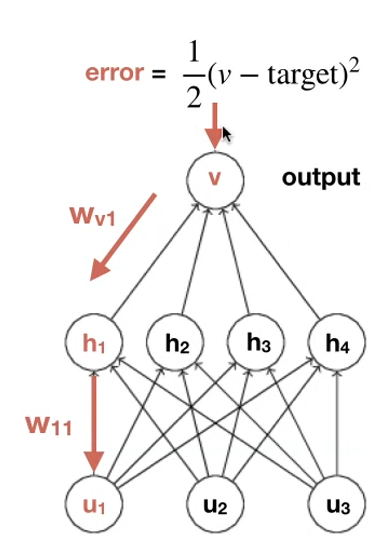
\includegraphics[scale=.5]{pics/backprop.png}
\end{center}

\textbf{Backpropagation} is typically used to perform gradient descent optimisation, adjusting the weights of neurons while optimising a desired loss function (error).

The backpropagation algorithm first calculates forward activity. The output is $v = W_vh$ (linear activation for $v$), and hidden layer is $h=f(W_uu)$ where $f$ denotes the activation function which is typically modelled as sigmoid or Rectifying linear unit function (ReLU).

Next, it calculates \textbf{error}. The error signal is typically modelled as:
\begin{align*}
\frac{1}{2} (v- \text{target})^2
\end{align*}

Finally, we \textbf{backpropagate} this error (how to calculate this gradient with respect to $w_{11}$):
\begin{align*}
\frac{\delta \text{Error}}{\delta w_{11}} = - \eta \frac{\delta \text{Error}}{\delta w_{11}} \frac{\delta v}{\delta h_1} \frac{\delta h_1}{\delta w_{11}}
\end{align*}

Resulting in:
\begin{align*}
\Delta w_{11} = -\eta \frac{\delta \text{Error}}{\delta w_{11}} = (v- \text{target}) w_{v1} f'_{h_1}u_1
\end{align*}

Unfortunately, at first glance, backpropagation in the brain does not seem to be biologically plausible. The key issues are:
\begin{enumerate}
\item Weight transport problem: Suggests that feedback weights = feedforward weights
\begin{itemize}
    \item The chain rule predicts feedback weights that are equal to feedforward weights, but there is no evidence that feedback connections exactly mirror feedforward ones
    \item The solution to this remains unclear, but it has been found that exact feedback weights can be replaced by random weights, without a major impact on performance. This method is known as feedback alignment and suggests that the brain may not need an exact feedback signal to implement `backprop'.
\end{itemize}
\item Derivative of activation functions: relies on calculating derivatives of activation functions
\begin{itemize}
    \item Backprop relies on the derivative of the activation function, but it is not clear how neurons could calculate their own derivative.
    \item The solution to this is also unclear, but as long as the gradient direction is not impacted, the derivative is not critical for performance.
\end{itemize}
\item Two phase learning: feedforward propagation of activity and error backpropagation
\begin{itemize}
    \item Backprop relies on two phases, a feedfoward pass of activity and then a backpass of errors. In the brain, there is no clear separation between perception and learning.
\end{itemize}
\item Separate error network: Suggest the need for a separate biological network computing the learning rules
\begin{itemize}
    \item The chain rule in backprop can be seen as a separate network, but there is minimal evidence for the existence of such gradient or error networks.
\end{itemize}
\item Non-local learning rules: The weight update depends on non-local information
\begin{itemize}
    \item Backprop relies on non-local learning rules, but learning is believed to occur through local changes at synapses, which is a process known as synaptic plasticity which can only access locally available information.
\end{itemize}
\item Target: the target label guides supervised learning.
\end{enumerate}

\subsubsection{Pyramidal cells}
We will now take inspiration from real neurons (pyramidal cells). These are one of the most common neurons in the brain.

\begin{center}
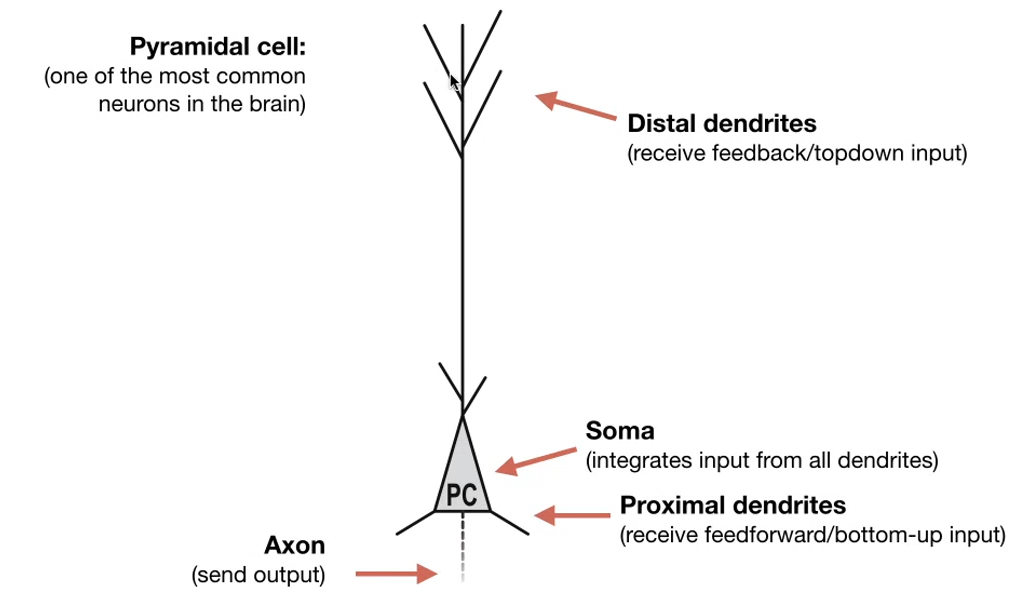
\includegraphics[scale=.3]{pics/pyramidal-cell.png}
\end{center}

The the brain, we have multiple areas, each made up of multiple pyramidal cells. This is the inspiration from which we get our new models of computer representations of learning in the brain. There are two cell types in the cortex, \textbf{Pyramidal} cells (excitatory cells) and \textbf{Martinotti} cells (inhibitory cells). These two work together. 

Dendritic microcircuits are those that approximate backpropagation, and look like this (NOTE!: $u$ and $v$ have a different meaning from before!):

\begin{center}
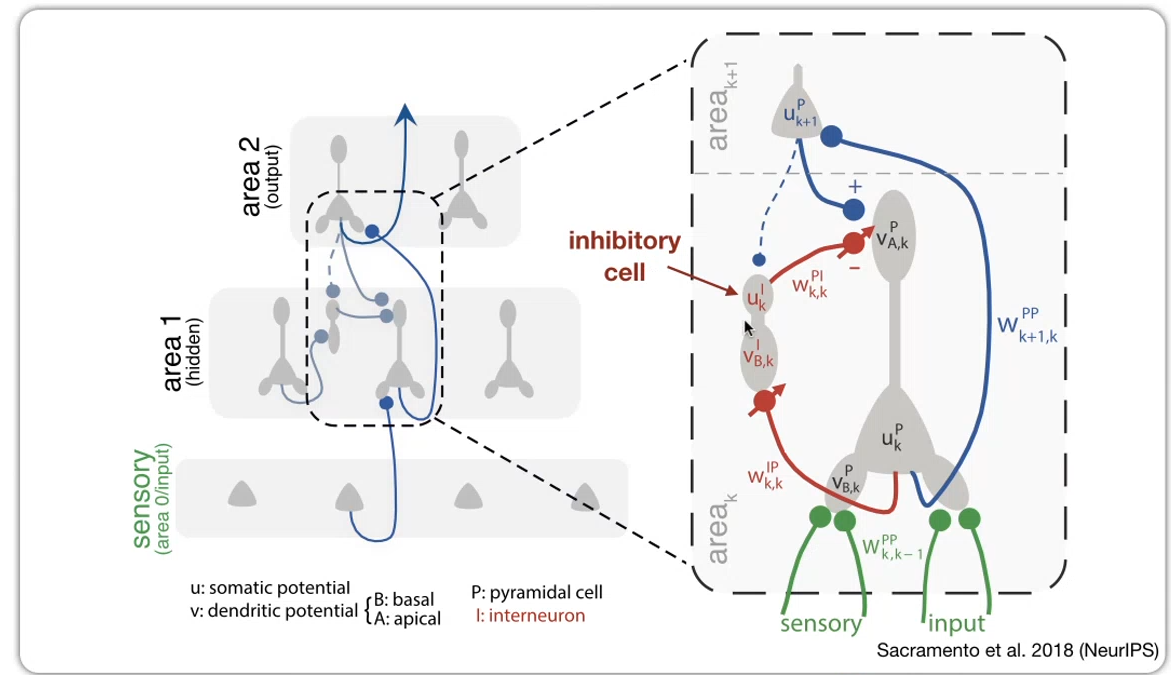
\includegraphics[scale=.4]{pics/dendritic.png}
\end{center}

The general idea of this is the difference between the topdown activity from $u_{k+1}^P$ and lateral inhibition $u_k^I$ generates an \textbf{error} signal: $v_{A,k}^P \sim u_{k+1}^P - u_k^I$

The \textbf{error} signal triggers changes in bottom weights $w_{k,k-1}^{PP}$.

The model learns recursively across areas/layers (just like in backprop) to correctly predict an output. During this process, lateral inhibition learns to predict the top-down input, leading to a zero error after learning, i.e.: $u_k^I \sim u_{k+1}^P$

The general form of the local learning rule is
\begin{align*}
\frac{d}{dt}w \sim \eta (u-v)r
\end{align*}

Where:
\begin{itemize}
    \item $u$: somatic activity
    \item $v$: input
    \item $\eta$: learning rate
    \item $r$: presynaptic activity
\end{itemize}

The learning rule for the bottom-up synapses is:
\begin{align*}
\frac{d}{dt}w_{k,k-1}^{PP} \sim \eta (u_{k+1}^P - u_k^P)r_{k-1}^P
\end{align*}

Note that this is really similar to the backprop learning rule:
\begin{align*}
\Delta w^{PP} \sim \eta \text{ error}_k \ r_{k-1}^p
\end{align*}

By being closer to biology, we were able to solve three of the key problems we discussed above:
\begin{itemize}
    \item Two phase learning: No need to two separate phases
    \item Separate error network: Neuron encodes both activity and errors
    \item Non-local learning rules: learning is local
\end{itemize}

Finally, if we look at the problem of the \textit{target} we know that backprop needs a specific target (or \textit{teaching signal}). It is really hard to imagine how the brain would be able to do this. One solution is that backprop works in unsupervised learning, so we can use that. Another solution is that specific brain areas may be calculating teaching signals that are used for internal supervised learning at other brain areas.

\subsubsection{Supervised learning in the Cerebellum}
The \textbf{cerebellum} has a stereotypical structure and contains more neurons than the rest of the brain. It is typically involved in motor error correction, but growing evidence suggests that it is also involved in regulating many other aspects of behaviour.

It seems to use a form of supervised learning but may also provide teaching signals to the cerebral cortex. So, the cerebellum can be used as an adaptive filter or controller. 

The cerebellum's circuit looks really similar to reinforcement learning, because the forward model has a prediction that it compares with the outcome.

The fact that the cerebellum has so many neurons leads us to believe that it could be used in much more than simple motor control. A 2D cognitive map of the cerebellum shows that there is activation to many different tasks.

\subsubsection{Summary}
In summary:
\begin{itemize}
    \item Deep learning successes rely on the backprop algorithm.
    \item Backprop is slowly becoming a possible model for learning in the brain, but several key issues remain unsolved.
    \item Dendritic microcircuits provide a powerful model of learning in the brain that approximates backprop.
\end{itemize}

\section{Visual System and Learning}
Our visual system works by projecting the image of the world onto the back of the eye (the retina) which is then relayed by the optic tract and sent to the visual cortex at the back of the brain. We can then record individual neurons and hope they respond to the visual stimulus presented to the brain.

The visual cortex has a few sub-areas. The primary visual cortex, the secondary visual cortex, and the inferior temporal cortex. The visual cortex also has receptive field which is a region of sensory space in which as stimulus modifies the firing rate of the neuron. The simple model of a receptive field is just a grid (visual input, $u$). This is then relayed via weights ($w$) to the visual cortex neuron ($v$), giving us this familiar equation $v = f(wu)$.

\subsection{Simple cells}
A \textit{simple cell} is a representation of a cell in the primary visual cortex. We can give a test subject a certain orientation of a white bar on a black background and see which neurons react to the particular stimulus on a particular location. If the bar is moved, the neuron might not respond as much, or might be a bit delayed. If the bar orientation is moved, the neuron may not fire at all.

The classic model for a simple receptive field (as seen in simple cells) is a \textbf{gabor filter}:
\begin{align*}
w \sim g(x,y;\lambda, \theta, \phi, \gamma) = \exp \bigg ( - \frac{x'^2 + \gamma ^2 y'^2}{2\sigma^2}\bigg) \cos \bigg ( 2\pi \frac{x'}{\lambda} + \phi \bigg)
\end{align*}

where:
\begin{itemize}
    \item $x,y$ are coordinates
    \item $\sigma$ is the standard deviation
    \item $\gamma$ defines the aspect ratio. If $\gamma = 1$, then the kernel is very circular. If $\gamma \sim 0$, then the kernel is elliptical in one direction, and almost 0.
    \item $\theta$ is wavelength
    \item $\phi$ is the phase offset
\end{itemize}

A Gabor filter is a product of a \textit{Gaussian} and \textit{sinusoid} that can model a periodic pattern similar to simple cells. 

\subsection{Complex cells}
Complex cells are able to fire neurons even if the stimulus is moved. However, if the orientation changes, it stops responding. Complex cells can be modelled as a set of simple cells with the same orientation but different locations, and simple cells can be modelled with Gabor Filters.

Generally speaking, simple cells are encoded in lower levels, such as V1, while complex cells are encoded higher up in places like V2. As you go higher and higher, you can have more complex components, such as edge cells (that encode edges) or even face cells (that encode faces).

\subsection{Grandmother cell}
This leads us to the concept of a grandmother cell. The idea here is that there are neurons responding specifically when you see people you are familiar with.

\subsection{Convolution Neural Networks}
CNNs can be used as a model of the visual system. This is a type of supervised learning, but the visual system is \textit{unsupervised}. CNNs along with backprop have revolutionalised computer vision nonetheless. The performance is unmatched.

The two key operations are:
\begin{itemize}
    \item Spatial convolution: Scanning the image with a filter
    \item Pooling: Subsampling input 
\end{itemize}

CNNs learn hierarchical features similar to the ones found in the brain.

\subsection{Summary}
\begin{itemize}
    \item The visual cortex is spread across multiple areas
    \item Receptive fields of increasing complexity
    \item Mathematical models of simple and complex cells
    \item CNNs as a representation of the visual system.
\end{itemize}

\section{Reinforcement Learning}
Reinforcement learning is the most common form of learning in the animal kingdom. The goal of this type of learning is to learn what actions to take maximise the rewards.

Some rewards are really sparse (such as winning or losing a game of something), and this poses a challenge because it's hard to realise what moves made should be rewarded since the final reward is the result of countless moves.

The general framework is the \textbf{Markov Decision Process}. In a basic form, this means that `the future is independent of the past, given the present'. Mathematically, t his can be defined as the following transition probability of the future given the immediate past:
\begin{align*}
P(S_{t+1}|S_t = P(S_{t+1}|S_1, \dots, S_t))
\end{align*}

It assumes that the current state $S_t$ has all the information needed to make a decision about the next state $S_{t+1}$.

In a Markov decision process, we define this by the following tuple:
\begin{align*}
(S,A,P,R,\gamma)
\end{align*}

Where:
\begin{itemize}
    \item $S$: Set of states
    \item $A$: Set of actions
    \item $P$: Transition probability $P^a_{ss'} = \mathbb{P}(S_{t+1} = s' | S_t = s, A_t = a)$
    \item $R$: Reward function $R^a_s = \mathbb{E}(T_{t+1} = s' | S_t = s, A_t = a)$
    \item $\gamma$: Discount factor $[0,1]$. This is usually set to $0.9$ so the system slowly forgets the previous rewards
\end{itemize}

The goal is the find the \textbf{policy} that finds the maximises \textbf{discounted reward}.

A policy is the distribution over actions given states. It defines the behaviour of an agent:
\begin{align*}
\pi(a|s) = P(A_t = a | S_t = s)
\end{align*}

A discounted reward is the total discounted reward received by the agent:
\begin{align*}
R_t = r_t + \gamma r_{t+1} + \gamma^2 r_{t+2} + \dots = \sum_{t=0}^{\infty} \gamma^t r_t
\end{align*}

It is useful to define the \textbf{value} of a state as the expected cumulative reward:
\begin{align*}
V^\pi (s) = \mathbb{E} \Bigg [ \sum_{t=0}^{\infty} \gamma ^t r_t | s_0 = s, \pi \Bigg]
\end{align*}

For that we have the \textit{Bellman equation} which gives the expectatino over the policy for $t$ and $t+1$:
\begin{align*}
V^\pi (s) = \mathbb{E}_\pi [r_t + \gamma V^\pi (S_{t+1}) | S_t = S]
\end{align*}

\subsection{Temporal Difference (TD) Learning}
\textbf{TD Learning}: is model-free reinforcement learning method that learns by bootstrapping based on current value function estimates. From the \textit{Bellman equation}, we get an iterative method for updating hte value function:
\begin{align*}
V(S_t) = V(S_t) + (R_{t+1} + \gamma V(S_{t+1}) - V(S_t))
\end{align*}

This gives us an estimate for the future rewards.

\begin{tcolorbox} [space to upper,
collower=white,
title={Tabular TD(0) for estimating $v_\pi$},
nobeforeafter,
halign lower=flush right, ]
Input: the policy $\pi$ to be evaluated.

Algorithm parameter: step size $\alpha \in (0,1]$

Initialise $V(s)$ for all $s \in S^+$, arbitrarily except that $V(terminal) = 0$

Loop for each episode:
\begin{itemize}
    \item Initialize $S$
    \item Loop for each step of episode:
    \begin{itemize}
        \item $A \leftarrow$ action given by $\pi$ for $S$
        \item Take action $A$, observe $R,S'$
        \item $V(S) \leftarrow V(S) + \alpha[R + \gamma V(S') - V(S)]$
        \item $S \leftarrow S'$
    \end{itemize}
    \item Until $S$ is terminal
\end{itemize}
\end{tcolorbox}

\subsection{Q-Learning}
Another example of reinforcement learning is Q-Learning. Here, we learn an action-value function:
\begin{align*}
Q(S_t,A_t) = Q(S_t,A_t) + R_{t+1} + \gamma \max_a Q(S_{t+1}, a) - Q(S_t,A_t)
\end{align*}

\begin{tcolorbox} [space to upper,
collower=white,
title={Q-Learning for estimating $\pi \simeq \pi$},
nobeforeafter,
halign lower=flush right, ]
Algorithm parameters: step size $\alpha \in (0,1]$, small $\epsilon > 0$

Initialise $Q(s,a)$ for all $s \in S^+, a \in \mathcal{A}(s)$, arbitrarily except that $Q(terminal,\cdot) = 0$.

Loop for each episode:
\begin{itemize}
    \item Initialise $S$
    \item Loop for each step of episode:
    \begin{itemize}
        \item Choose $A$ from $S$ using policy derived from $Q$ (such as $\epsilon$-greedy)
        \item Take action $A$, observe $R,S'$
        \item $Q(S,A) \leftarrow Q(S,A) + \alpha[R + \gamma \max_aQ(S', a) - Q(S,A)]$
        \item $S \leftarrow S'$
    \end{itemize}
    \item Until $S$ is terminal
\end{itemize}
\end{tcolorbox}

The main difference is that we use the \textbf{best action} in the next state ($\max_aQ(S',a)$). Other than this, the two algorithms are very similar. TD-Learning uses the value of the \textbf{state given} by the policy, while Q-learning uses the \textbf{best possible action}, not necessarily the one given by the policy.

\subsection{Bigger spaces}
What if we have something with hundreds or millions of states? Possible solutions include:
\begin{itemize}
    \item Using exploration-exploitation strategies
    \item Use function approximates (e.g. neural rewards)
\end{itemize}

There is an \textbf{exploration-exploitation} tradeoff where \textbf{exploitation} makes the best decision given current information and \textbf{exploration} gathers more information. The classic policy that relies on this tradeoff is the $\epsilon$-greedy policy, which is a policy for when to choose the best available action $a*$ or a random action:

\begin{align*}
a_t = \bigg \{
\begin{matrix} 
    a_t^*                  & \text{with probability } 1 - \epsilon \\
    \text{random action } & \text{with probability } \epsilon
\end{matrix}
\end{align*}

\begin{itemize}
    \item $\epsilon=1$ gives a purely exploratory policy
    \item $\epsilon=0$ gives a purely exploitative policy
    \item $\epsilon=]0,1[$ gives somewhere in-between these two ideas. It is generally a good idea to explore more in the beginning and then exploit more towards the end of the optimisation.
\end{itemize}

\subsection{Deep Q-learning}
Recent success in reinforcement learning relies on two tricks:
\begin{enumerate}
\item Use neural network as $Q(S,A;\theta)$ function approximator with parameters $\theta$
\item Use separate memory system to avoid getting stuck at local optima
\end{enumerate}

\section{Unsupervised Learning}
Most sensory data we receive is of the unsupervised variety. There is no teaching signal and no feasible reward for every bit of data.

\subsection{Sparse Coding}
Sparse coding is a form of encoding in networks. It's where you only have a small set of units responding for a given input. It provides a framework for learning sparse representations of the input.

The actual \textit{definition} is that sparse coding is the representation of items by the strong activation of a relatively small set of neurons. For each stimulus, this is a subset of all available neurons

Sparse coding has these key properties:
\begin{itemize}
    \item \textbf{Overcomplete dictionary W}: $d>m$ (i.e. more dictionary elements than input elements)
    \item \textbf{Sparseness}: Number of zero elements in $v$ is much larger than then number of non-zero elements
    \item Overcomplete and sparse representation leads to \textbf{richer features}.
\end{itemize}

These properties are represented in the cost function, where we have the convention of two important terms: \textit{preserve information} and \textit{sparseness}. The cost function looks like this:
\begin{align*}
\text{cost } = [\text{preserve information}] + \lambda [\text{sparseness}]
\end{align*}

Sparse coding with L1 norm is:
\begin{align*}
\arg \text{min}_{W,V} = ||U-WV||^2_2 + \lambda ||V||+1
\end{align*}

\begin{itemize}
    \item To find a good sparse code, we need to optimise both the dictionary $W$ and the representation $V$.
    \item This optimisation is convex in $V$ and $W$ separately, but not both.
    \item Several methods exist to optimise $V$ and $W$, but we will only discuss one
    \item $\lambda$ controls the tradeoff between sparseness and reconstruction.
\end{itemize}

Sparse coding is really good for noise reduction of an image or image restoration.

In the visual system, this is an easy mapping from conceptual to real. The inputs are mapped to the \textbf{LGN}, that is a region between the retina and the back of the brain. This input goes through some set of weights (maps to our $W$). Finally, the visual cortex itself is the output.

\subsection{Sparse Coding in the Brain}
We are now going to look at one type of cost function:
\begin{align*}
\text{argmin}_{W,V} = ||U-WV||^2_2 + \lambda \sum_{i}S(v_i)
\end{align*}

Where $S(v_i) = \log(1+v_i^2)$.

We need to derive a way to optimise these two sets of components, as discussed previously. Let's start with $V$.
\begin{align*}
w_iU - \sum_{j \not = i} G_{ij}v_j - f_\lambda(v_i)
\end{align*}

where $G_{ij} = w_i w_j$ and $f_\lambda(v_i) = v_i + \lambda S'(v_i)$.

Secondly, we need to optimise the weights as
\begin{align*}
\Delta w_i &= \eta \frac{\delta \text{Cost}}{\delta w_i} \\
&= \eta < [U- \hat U]v_i > \\
&= \eta < [U - \sum_{i}^{m}w_iv_i]v_i >
\end{align*}

The learning rule is local and there is a Hebbian term ($UV$ meaning a function of pre and post synaptic connectivity) and a postsynaptic only term ($WV^2$ that causes decay).

Sparse coding is really useful for the brain because it has good representations of information that can be used for decision making and discrimination. It's also really energy efficient, with only a few neurons active at a given time. Finally, it's also more robust to peturbations than purely localist codes.

\subsection{Autoencoders}
Autoencoders are very popular and use a similar cost function to the one discussed above. We give a network an input and then the network learns a sparse or compressed representation of the input. There is a network \textit{bottleneck}, after which the network starts to decode the network. It essentially goes from lots of nodes, to few nodes (which is the bottleneck), and finally up to many (the re-representation).

The aim is to reconstruct the input, but without an explicit constraint on sparsity, and instead on other forms of regularisation.

The cost function for this, therefore is:
\begin{align*}
\text{argmin}_W = ||V_U||^2_2
\end{align*}

\section{Temporal processing and Recurrent Neural Networks (RNNs)}
Temporal processing is crucial for our perception of the world. For example, with speech, you obviously are unable to understand things that are backwards (like reversed). The content of two clips where one is reversed is technically the same.

\subsection{Temporal Processing}
We have a few brain areas that are key for language processing in the brain. \textbf{Broca's area} is particularly important for speech production, while the many other cortices are used for speech understanding. I don't think this will be necessary content for the exam, but if it is, check the first part of lecture 6.

Receptive fields are also present for natural sounds in the auditory cortex, similar to the way that natural shapes are seen in the visual cortex. Receptive fields for audio seem to be localised in time and frequency domains, also similar to those in the visual cortex.

Feedforward networks do not model time \textit{explicitly}. One option is to consider each input as being a different time point, but this is still quite hacky, because it is not how the brain work and does not seem to be a natural solution to the problem. Instead, in a \textbf{recurrent network}, each node is \textit{laterally connected} and is also able to be connected to itself (have some memory about previous input). 

We would model discrete time (the next time point $v_{t+1}$) as:
\begin{align*}
v_{t+1} = rv_t + f(Wu_t + Mv_t)
\end{align*}

Here:
\begin{itemize}
    \item $r$ is the activity delay
    \item $u$ is the feed forward input
    \item $M$ is the recurrence input from other units
\end{itemize}

Furthermore, we can model continuous time as
\begin{align*}
\tau_r \frac{dv}{dt} = -v + f(Wu + Mv)
\end{align*}

Here:
\begin{itemize}
    \item $dv/dt$ is the modelling of change in $v$ over time
    \item $\tau_r$ controls this and is the timeconstant of activity decay
    \item $-v$ is the passive decay
    \item The rest is the same as the discrete case
\end{itemize}

\subsection{Recurrent Neural Networks (RNNs)}
An application of RNNs in neuroscience is that the brain remembering where it is looking at despite constant blinking. Is there some sort of memory for this? Remembering eye position seems to be encoded by three neurons. One encodes the direction clockwise, and the other counter clockwise. When the eye changes direction, one of these two neurons fire. There is a third neuron called an \textit{integrator} neuron, that fires the whole time, and the rate determines where the eye is. The integrator gets input from the \textbf{on} and \textbf{off-direction} neurons resulting in an eye position. This integrator is related to the discrete time model equation discussed above.

\begin{itemize}
    \item For $r=1$ we have a perfect integrator, where the neuron remembers previous inputs forever
    \item For $r<1$ the activity decays back to baseline
    \item For $r>1$ the activity grows exponentially over time
\end{itemize}

So you choose or optimise $r$ depending on the timescale of memory you need for a given task.

Some networks use a \textbf{winner-takes-all} network, which is similar to applying a \textit{max} operator on the response of $k$ neurons. Using lateral inhibitory neurons is a way of implementing such a max operation in a network. If we don't have this winner takes all, we might have multiple neurons firing for a certain eye position, but applying this means we only have a single, strongest neuron firing.

\subsubsection{Attractor Neural Networks}
Attractor neural nets are another form of RNN modelled as dynamic systems that contain a number of attractor states with low energy to which the network dynamics converge. An example of this is the \textbf{Hopfield} network.

These attractor neural nets have two key properties:
\begin{itemize}
    \item $m_{ii} = 0$: no unit has a connection with itself
    \item $m_{ij} = m_{ij}$ connections are symmetric
\end{itemize}

There is also a stochastic version of the Hopfield network, called a \textbf{Boltzmann machine}. The total input is
\begin{align*}
z_i = b_i + \sum_{j}^{\text{external input}} u_jw_{ij} + \sum_{x}^{\text{recurrent input}} v_x m_{ix}
\end{align*}

The probability of turning on a given neuron $i$ is
\begin{align*}
P_{i=on} = \frac{1}{1 + \exp (-\frac{z_i}{T})}
\end{align*}

If temperature $T = 0$, we just get a Hopfield network.

Boltzmann machines are good generative models, meaning they are able to recreate shapes pretty well when they have learned it.

\subsection{Reservoir computing}
Reservoir computing uses a large pool of sparsely connected neurons that generate a large repertoire of dynamics (they have \textit{fading memory}) and learn a simple read-out to combine the interesting dynamics into a useful output.

There are two specific variants of reservoir computing: \textbf{echo state networks} and \textbf{Liquid state machines}

Echo state networks is the most common \textit{rate-based} (meaning neurons are modelled at the level of firing rates) reservoir networks.

Liquid state machines are similar to echo state machines, but neurons are modelled at the level of individual spikes, which is a more realistic estimation of neurons.

\subsection{Recurrent CNNs}
Most brain areas exhibit a high degree of recurrence. Recent developments show that if CNNs are extended with specific forms of recurrence, they are able to outperform purely feedforward CNNs.

\section{Microcircuits and RNNs}
We have two umbrella types of neurons in the brain: \textit{inhibitory} and \textit{excitatory} neurons. The activity between these two is very balanced, which is good because it means that there is no runaway activity.

The inhibitory learning rule is:
\begin{align*}
\Delta w_{\text{inh}} &= \eta x (y - r_0) \\
0 &= \eta x(y-r_0) \\
y &= r_0
\end{align*}

Where $r_0$ is the target rate of the post synaptic neuron $y$. $r_0$ is typically quite a low number.

What we have seen from inhibitory plasticity is that inhibition learns to follow excitation. It means that the receptive fields are balanced.

Inhibitory cells come in different flavours. Pyramidal cells are one type of inhibitory cell, but together with these, there are multiple more types. We won't talk about all these, but it's important to know. We will be looking at \textbf{basket cells}, which make up around 50\% of the inhibitory neurons in the brain.

\subsection{Long Short-Term Memory (LSTM)}
LSTMs are the state of the art recurrent neural network model. They are useful because they are gated neural network that is able to capture both short and long term data. At the heart of this network is the memory cell.

\begin{center}
    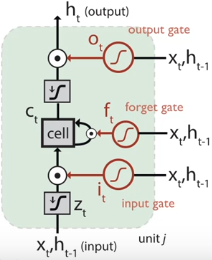
\includegraphics[scale=.7]{memory_cell.png}
\end{center}

This structure very closely resembles the circuits we see in the \textit{cortical circuits}. There is an important difference, however. We do the gating with \textit{multiplicative difference} in LSTM, but in neuroscience, we often interpret this gating as being inhibitory, meaning it should be subtractive. This moves us to a new model, \textbf{sub-LSTM}, where the gating is subtractive.

\subsection{Summary}
\begin{itemize}
    \item Multiple excitatory and inhibitory cell types in the brain
    \item Intricate microcircuits across multiple layers
    \item Machine learning LSTMs are a form of gated-RNN good for capturing long-term dependencies such as language modelling
    \item Cortical microcircuits have similar features to gated-RNNs but may operate with subtractive gating (subLSTMs)
\end{itemize}
\end{document}